\chapter{Radioactivité $\beta$}
\section{Définitions}
On s'intéresse ici à ce qui se passe dans le noyau, c'est-à-dire que le nombre de nucléons ne sera pas modifié. La
différence de masse $m_{neutron}-m_{proton} = 1.3$ MeV implique que le proton instable mais pas le neutron. La 
radioactivité $\beta$ est un processus pù
\begin{itemize}
\item[$\bullet$] Un neutron est converti en proton : $n\to p+e^-+\bar nu$
\item[$\bullet$] Un proton est converti en neutron : $p\to n+e^++ nu$
\end{itemize}\ 

Il faut qu'il y ai conservation du nombre leptonique (0=0+1-1), du moment cinétique et de l'énergie (le spectre
des électrons est continu). Or, ceci n'était pas vrai si un neutron se changeait "juste" en proton ou inversement. 
C'est pour ça que \textsc{Pauli} a émis l'hypothèse de l'existence du \textit{neutrino} en \textit{1931}, une
particule de spin 1/2 (fermion) et de masse presque nulle interagissant peu avec la matière (si peu que la détection
n'a été rendue possible qu'en \textit{1950}).\\

Il y a d'autres processus lié à la radioactivité $\beta$ : la capture électronique ($p+e^-\to n+\nu$), la 
capture positronique ($n+e^++\to p+\bar\nu$) (pas observée) et l'émission de leptons lourds ($\mu, \tau$) mais 
celle-ci ne se déroule pas dans les noyaux (et on n'en parlera pas, cf. le nom du cours).

\section{Transition $\beta$ dans les noyaux}
Ces transitions ne modifient donc pas le nombre total de nucléons. Elle se manifeste (dans ce cours) sous 
trois aspect
\begin{description}
\item[Transition $\beta^-$]  Un neutron est transformé en proton avec émission (conservation de la charge) d'un 
électron et d'un anti-neutrino (conservation du nombre leptonique et de l'énergie. Si on émet une particule il
faut également une antiparticule). Ceci concerne les isotopes \textit{en-dessous} de la vallée de stabilité qui ont
un excès de neutrons.
\begin{equation}
^A_ZX_N \to A_{Z+1}Y_{N-1} + e^- + \bar \nu
\end{equation}
\item[Transition $\beta^+$] Concerne les isotopes \textit{au-dessus} de la vallée de stabilité, ceux-ci ayant un
excédent de proton. Par $\beta^+$, on revient vers celle-ci (parabole de masse)
\begin{equation}
^A_ZX_N \to A_{Z-1}Y_{N+1} + e^+ + \nu
\end{equation}
\item[Capture électronique] Phénomène allant en parallèle avec $\beta^+$ car ils vont souvent ensemble. La différence
est que la capture donne un spectre \textbf{mono}énergétique (comme $\alpha$) car il n'y a que deux particules 
(s'il y en a trois, la répartition de l'énergie entre deux donne un continuum).
\begin{equation}
^A_ZX_N +e^- \to A_{Z-1}Y_{N+1}^*  + \nu
\end{equation}
\end{description}

\subsection{A. Bilans nucléaires}
Nous allons regarder le bilan d'énergie qui sera ici plus compliqué car il faut tenir compte de la différence
de masse du neutron et du proton, mais également que leur nombre change. Notons que les bilans sont ici 
nucléaires (le nuage électronique est négligé).

\subsubsection{Transition $\beta^-$}
Partons d'un état d'initiale avec une certaine masse exprimée avec l'énergie de liaison $B$
\begin{equation}
m(A,Z) = Zm_pc^2 + Nm_nc^2 - B(A,Z)
\end{equation}
Il faut tenir compte des énergies cinétiques pour l'état final 
\begin{equation}
m(A,Z+1) +m_ec^2+T_e+T_\nu = (Z+1)m_c^2+(N-1-m_nc^2-B(A,Z+1)+m_ec^2+T_e+T_\nu
\end{equation}
Par conservation de l'énergie
\begin{equation}
T_e+T_\nu = Q_{\beta^-}^N = B(A,Z+1)-B(A,Z)+\underbrace{(m_n-m_p-m_e)c^2}_{0.782\text{ MeV}}
\end{equation}
La quantité $ Q_{\beta^-}^N$ (seuil) doit être positive afin que la transition soit possible. L'électron et 
le neutrino se partagent l'énergie de seuil donnant un spectre continu (trois corps).


\subsubsection{Transition $\beta^+$}
En suivant un résultat analogue, on trouve pour le seuil
\begin{equation}
Q_{\beta^+}^N = B(A,Z-1)-B(A,Z)-\underbrace{(m_n-m_p-m_e)c^2}_{1.804\text{ MeV}}
\end{equation}
La différence vient du fait que neutron et proton n'ont pas exactement la même masse.


\subsection{Bilans atomiques}
Prenons cette fois-ci en compte les électrons. 

\subsubsection{Transition $\beta^-$}
	\begin{wrapfigure}[9]{r}{7cm}
%	\vspace{-5mm}
	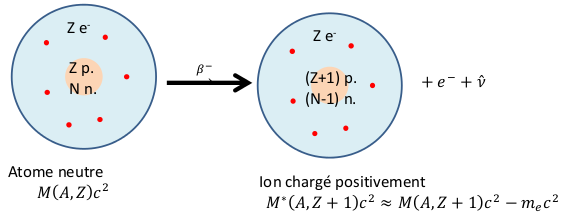
\includegraphics[scale=0.4]{ch6/image1}
	\captionof{figure}{ }
	\end{wrapfigure}

Dans l'état initial, l'atome est neutre : $Z$ protons, $N$ neutrons et $Z$ électrons formant un cortège 
électronique. L'état final est un ion positif : $Z+1$ protons, $N-1$ neutrons et $Z+1$ électrons. Le seuil 
atomique est donné par
\begin{equation}
\begin{array}{ll}
Q_{\beta^-}^a &= M(A,Z)c^ 2 - [M^*(A,Z+1)c^2+m_ec^2]\\ &\approx M(A,Z)c^2+M(A,Z+1)c^2
\end{array}
\end{equation}
où nous avons négligé l'énergie d'ionisation de l'électron.

\newpage
Comparons les deux seuils (atomique et nucléaire)
\begin{equation}
Q_{\beta^-}^a \approx M(A,Z)c^2-M(A,Z+1)c^2,\qquad\qquad
Q_{\beta^-}^N = m(A,Z)-m(A,Z+1)-m_ec^2
\end{equation}
On comparaison avec le seuil nucléaire $M(A,Z)c^2 = m(A,Z)+Zm_e+B_e$. Dès lors, si les énergies de liaison 
$B_e$ sont proches dans les états initial et final, nous avons que $Q_{\beta^-}^a\approx Q_{\beta^-}^N$. Ceci
n'est pas toujours vrai comme le montre le $^{187}$Re (voir \textit{slide 78}).



\subsubsection{Transition $\beta^-$}
	\begin{wrapfigure}[9]{r}{7cm}
%	\vspace{-5mm}
	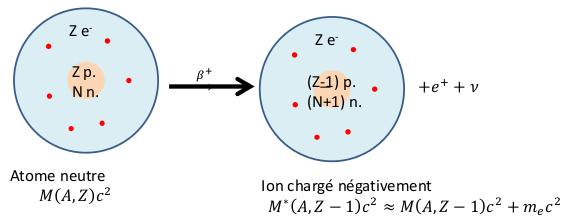
\includegraphics[scale=0.4]{ch6/image2}
	\captionof{figure}{ }
	\end{wrapfigure}
Les signes changent mais l'idée est la même. Dans l'état initial, l'atome est neutre : $Z$ protons, $N$ neutrons 
et $Z$ électrons formant un cortège électronique. L'état final est un ion négatif : $Z-1$ protons, $N+1$ neutrons 
et $Z$ électrons. Le seuil 
atomique est donné par
\begin{equation}
\begin{array}{ll}
Q_{\beta^+}^a &= M(A,Z)c^2 - [M^*(A,Z-1)c^2+m_ec^2]\\ &\approx M(A,Z)c^2+M(A,Z-1)c^2-2m_ec^2
\end{array}
\end{equation}
où nous avons négligé l'énergie d'ionisation de l'électron.

\subsubsection{Capture électronique}
	\begin{wrapfigure}[14]{l}{8.5cm}
	\vspace{-5mm}
	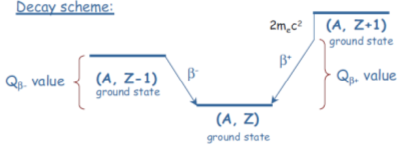
\includegraphics[scale=0.55]{ch6/image3}
	\captionof{figure}{Parabole de masse (gauche $\beta^-$, droite $\beta^+$). Le seuil $Q_{\beta^+}$ n'est
	 pas simplement la différence de masse mais celle différence soustraite de $2m_ec^2$. Cette compétition ne
	 concerne que $\beta^+$. Le seuil différent implique que certaines transitions ne sont que de type CE.}
	\end{wrapfigure}

La capture électronique est un phénomène qui rentre en compétition avec $\beta^+$ où un électron du cortège
électronique est capturé pour former un noyau dans lequel un proton est transformé en neutron. 
\begin{equation}
^A_ZX_N+e^-\to ^A_{Z-1}Y^*_{N+1}+\nu
\end{equation}
où le cortège électronique est excité. Ici les neutrinos sont monoénergétique (ce qui n'est \textbf{pas} le cas
pour la désintégration $\beta^\pm$). Ce phénomène est par contre impossible pour un atome complètement isolé.
Si cela va "ensemble" avec $\beta^+$, c'est parce que le même noyau est produit à partir du même noyau initial. 
La différence importante, ce sont les seuils (différence de masses avec une petite correction $\Delta_{el}$ souvent
négligeable) qui diffèrent de $2m_ec^2$. En effet, le bilan final donne
\begin{equation}
Q_{CE} = M(A,Z)c^2-M(A,Z-1)c^2-\Delta_{el}\approx Q_{\beta^+}^a + 2m_ec^2
\end{equation}
L'électron final fait donc partie du cortège électronique de $\Delta_{el}$ est l'énergie d'excitation de l'atome
$Y$ (proportionnel à l'énergie de liaison de l'électron capturé). Il y a formation d'un "trou" dans le couche
électronique de $Y$ causant une réorganisation du cortège électronique.\\

Considérons le spectre des électrons. Si on néglige l'énergie de recul (l'énergie cinétique du noyau fille $Y$), 
pour $\beta^\pm$ nous avons
\begin{equation}
Q_\beta = T_e+T_\nu
\end{equation}
L'électron et le neutrino se partage l'énergie libérée ce qui fait que l'énergie de l'électron varie de façon
continue de 0 à $Q_\beta$. L'énergie totale libérée vaut donc $E=m_e+Q\beta$. Pour la capture électronique, le
spectre des neutrinos est monoénergétique $Q_{CE} = T_\nu$.

\newpage
\begin{center}
	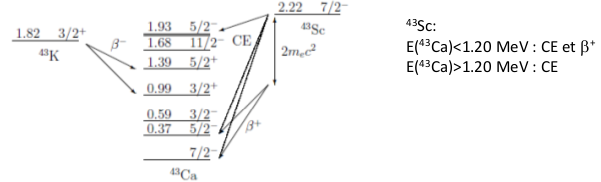
\includegraphics[scale=0.55]{ch6/image4}
	\captionof{figure}{Comme pour $\alpha$, il y a d'autres transitions que vers le fondamental pour autant que 
	les seuils soient respectés. Il y a compétition $\beta^+/CE$ mais la valeur de $2m_ec^2$ fait que l'on peut
	avoir du $\beta^+$ seulement en dessous de ce seuil et au dessus seulement de la capture électronique}
\end{center}\ 

\section{Théorie de Fermi}

\subsection{Généralités}
Cette théorie a été établie (de façon incomplète) en \textit{1934} en se basant sur l'analogie avec l'émission
d'un photon. Afin d'être précis, il y a nécessite de faire des calculs relativistes ($m_\nu\approx0, m_ec^2
\approx 0.511$ MeV). La règle d'or de \textsc{Fermi} permet d'estimer la probabilité de transition d'un état
vers un autre
\begin{equation}
\dfrac{dW}{dE} = \dfrac{2\pi}{\hbar}|V_{fi}|^2\rho(E)
\end{equation}
où $\rho(E) = \frac{dN}{dE_T}$ est la densité de niveaux à l'énergie $E_T=E_e+E_\nu$, d$\rho_\alpha(E) : 
\frac{(4\pi)^2}{(\hbar c)^2}(Q_\beta-T_e)^2k_e(T_e+m_ec^2)dT_e$ et $V_{fi}$ est l'élément de matrice de 
la transition $\beta$ que nous allons maintenant approfondir.

\subsubsection{Élément de matrice de transition $V_{fi}$}
Celui-ci est défini par
\begin{equation}
V_{fi}\equiv \bra{\Psi_f^N\Psi_e}G_FO_\beta\ket{\Psi_i^N\Psi_\nu}
\end{equation}
où $O_\beta$ est un opération de transition sans dimension et $G_F$ la constante de couplage de désintégration
$\beta$ (ou \textit{constante de Fermi}). Elle joue un rôle analogue à $e^2$ pour l'interaction électromagnétique 
(dimension $E\times L^3$). Elle est donnée par
\begin{equation}
G_F = m_ec^2\left(\frac{\hbar}{m_ec}\right)^3G_\beta
\end{equation}
où $G_\beta = 3.002\times 10^{-12}$. On retrouve également quatre fonctions d'ondes
\begin{enumerate}
\item[$\bullet$] $\Psi_i^N$, la fonction d'onde initiale nucléaire
\item[$\bullet$] $\Psi_f^N$, la fonction d'onde finale nucléaire
\item[$\bullet$] $\Psi_\nu$, la fonction d'onde du neutrino (selon la théorie des champ, l'apparition d'une 
antiparticule entraîne la disparition d'une particule)
\item[$\bullet$] $\Psi_e$, la fonction d'onde de l'électron
\end{enumerate}\ 

Pour rendre son traitement plus simple, on va la factoriser en une partie nucléaire et une partie leptonique
\begin{equation}
V_{fi} \approx G_F \bra{\Psi_f^N}O^N_\beta\ket{\Psi_i^N}\bra{\Psi_e}O^L_\beta\ket{\Psi_\nu}
\end{equation}
Pour la partie nucléaire, $M_{fi} = \bra{\Psi_f^N}O^N_\beta\ket{\Psi_i^N}$ doit être calculé à partir de 
modèles nucléaires.\\

La partie leptonique "provient" de l'intérieur du noyau. Comme le noyau est "petit" par rapport aux longueurs 
d'onde de l'électron et du neutrino (soit $\vec{r}$, la coordonnée commune de l'électron et du neutrino), on va
pouvoir faire quelques approximations. La première que que le neutrino n'interagit pas
\begin{equation}
\Psi_\nu \approx e^{i\vec{k}_\nu.\vec{r}}\approx1
\end{equation}
Un raisonnement similaire peut être tenu pour l'électron, mais celui-ci interagit avec les protons. Il faut donc
tenir compte de la fonction d'onde au voisinage de zéro (dépend de la charge du noyau)
\begin{equation}
\Psi_\nu \approx e^{i\vec{k}_e.\vec{r}}\Psi_e(0)\approx\Psi_e(0)
\end{equation}
Évaluons alors l'élément de matrice (via \textsc{Fermi})
\begin{equation}
|\bra{\Psi_e}O^L_\beta\ket{\Psi_\nu}|^2 \propto |\Psi_e(0)|^2|\Psi_\nu(0)|^2 = \frac{1}{(2\pi)^6}F(\pm Z, p_e)
\end{equation}
où l'on voit apparaître la fonction de \textsc{Fermi}, qui dépend de l'énergie (par le paramètre de 
\textsc{Sommerfeld}, $\eta$). Notons la normalisation de l'onde plane
\begin{equation}
\bra{e^{i\vec k.\vec r}}\ket{e^{i\vec k'.\vec r}} = (2\pi)^3\delta(\vec{k}-\vec{k}')
\end{equation}

\subsubsection{Fonction de Fermi}
	\begin{wrapfigure}[14]{l}{10.5cm}
	\vspace{-5mm}
	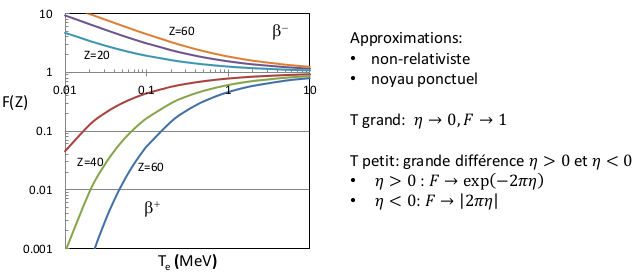
\includegraphics[scale=0.55]{ch6/image5}
	\captionof{figure}{ }
	\end{wrapfigure}
	
Dans un cadre non-relativiste, celle-ci s'écrit
\begin{equation}
F(\pm Z, p_e) : |\Psi_e(0)|^2 = \dfrac{2\pi\eta}{e^{2\pi\eta}-1}
\end{equation}\ \\
\\
\\

Celle-ci est toujours positive et dépend fortement de $Z$.  On y retrouve le \textit{paramètre de Sommerfeld}
qui "mesure" les effets coulombiens
\begin{equation}
\eta = \mp \dfrac{(Z\pm 1)e^2}{\hbar \nu}
\end{equation}
Pour l'émission $\beta^-$, $\eta <0$ et $F>1$, les électrons et le noyau s'attirent alors que pour l'émission
$\beta^+$, $\eta >0$ et $F<1$, les positrons et le noyau se repoussent.


\newpage
\subsubsection{Probabilité de transition totale}
En regroupant tous les différents termes
\begin{equation}
\frac{dW}{dE} = \dfrac{dW}{dT_e} = \frac{1}{2\pi^3}\frac{1}{\hbar(m_ec^2)^4}G_\beta^2cp_e(Q_\beta-T_e)^2(T_e+
m_ec^2)F(\pm Z,p_e)|M_{fi}|^2
\end{equation}
Nous avons bien une factorisation entre une partie purement nucléaire (via $M_{fi}$) et une partie
électronique (la fonction de Fermi dépend à la fois des propriétés électronique et du  noyau et le reste est 
purement électronique). Il existe une relation entre $T_e$ et $p_e$ :
\begin{equation}
E_e = \sqrt{(p_ec)^2+(m_ec^2)^2} = T_e+m_ec^2
\end{equation}

	\begin{wrapfigure}[11]{r}{5.5cm}
	\vspace{-5mm}
	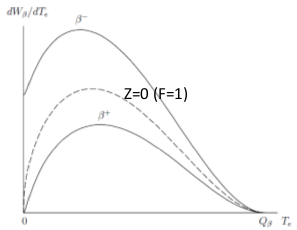
\includegraphics[scale=0.55]{ch6/image6}
	\captionof{figure}{ }
	\end{wrapfigure}
L'expérimentateur va mesurer $dW/dE$. Selon $\beta^\pm$, \textsc{Fermi} va réduire ou augmenter le spectre ce 
qui va causer une différence assez forte entre le spectre $\beta^+$ et le $\beta^-$. En effet $\beta^-$ est 
attiré par le noyau fille et $\beta^+$ repoussé ($T_e=0, F$ très petite).  Les comportement asymptotiques pour
$T_e=0$ sont
\begin{equation}
\beta^+ : F(\pm Z, p_e)\to 0,\qquad\qquad \beta^- : F(\pm Z, p_e)\to \frac{1}{\sqrt{T_e}}
\end{equation}
Notons que $dW/dE$ est non nul pour $T_e=0$. Comme annoncé ci-dessus, le spectre est continu pour des énergies 
entre 0 et $Q_{\beta}$. La durée de vie peut s'obtenir par intégration sur toutes les énergies cinétiques tandis
que la probabilité de transition totale est donnée par l'intégrale sur les énergies: $W = dW/dT_edT_e$ où 
$M_{fi}$ n'interviendra pas dans son calcul, étant un terme purement nucléaire.



\subsubsection{Élément de matrice nucléaire $M_{fi}$}
Celui-ci est défini par
\begin{equation}
|M_{fi}|^2 = B(F)+\lambda^2B(GT)
\end{equation}
On y retrouve la probabilité de transition réduite (elle même défini par deux opérateurs définissant les 
transitions $\beta$)
\begin{equation}
B(\sigma) = \dfrac{2J_f+1}{2J_1+1}|\bra{\Psi^{J_f\pi_f}}O(\sigma)\ket{\Psi^{J_i\pi_i}}|^2
\end{equation}
où $\Psi^{J_{i/f}\pi_{i/f}}$ sont les fonctions d'ondes du noyau dans l'état initial/final. On retrouve
aussi l'\textbf{opérateur de Fermi} $O(F)$ (à admettre)
\begin{equation}
O(F) = \sum_{i=1}^A t_{i,\pm} = T_\pm
\end{equation}
Il s'agit d'un OTI de rang 0 dans l'espace des spin et de rang 1 dans l'espace des isospins. Il ne dépend 
pas de $J$ mais seulement de l'isospin : il ne change pas par rapport au spin du noyau.\\

On trouve de même l\textbf{opérateur de Gamow-Teller} $O(GT)$
\begin{equation}
O(GT) = \sum_{i=1}^A \sigma_i t_{i,\pm}
\end{equation}
Qui est un OTI de rang 1 dans l'espace des spin et des isospin.\\

Les signes $\pm$ ci dessus signifient : + pour la radioactivité $\beta^+$ ($t_{i+}$ change un proton en un 
neutron) et - pour la radioactivité $\beta^-$ ($t_{i-}$ change un neutron en un proton).


\section{Règles de sélection}
\subsection{Transition de Fermi}
L'opérateur ne dépend pas du spin, il n'y a pas besoin de \textsc{Wigner-Eckaert}. Le spin initial doit
être le même que le spin final : $J_i=J_f$. Il ne dépend pas non plus de la parité, il doit être invariant
par réflexion (pair) : $\pi_i=\pi_f$. Il s'agit par contre d'un OTI de rang 1 dans l'espace des isospin. 
Regardons l'élément de matrice :
\begin{equation}
\bra{T'M_T'}T_\pm\ket{TM_T} = \sqrt{(T\mp M_T)(T\pm M_T+1)}\delta_{TT'}\delta(M_T'M_{T\pm1}
\end{equation}
Il faut que les $T$ soient identiques. De plus, l'opérateur $T_\pm$ change la projection (augmente ou diminue) 
mais pas la valeur du moment cinétique (isospin). En résumé
\begin{equation}
J_i=J_f,\qquad\qquad \pi_i=\pi_f,\qquad\qquad T_i=T_f
\end{equation}


\subsection{Transition de Gamow-Teller}
Cet opérateur est invariant par réflexion. l s'agit d'un OTI de rang 1 dans l'espace des spin mais aussi dans
celui des isospin. Il faut que
\begin{equation}
|J_i-J_f| \leq 1 \leq J_i+J_f,\qquad\qquad \pi_i=\pi_f, \qquad\qquad |T_i-T_f| \leq 1 \leq T_i+T_f
\end{equation}\ \\
\\
Afin d'avoir des transition de \textsc{Fermi} et \textsc{Gamow-Teller}, il faut que
\begin{equation}
J_i=J_f\neq 0,\qquad\qquad \pi_i=\pi_f,\qquad\qquad T_i=T_f\neq 0
\end{equation}

\begin{center}
	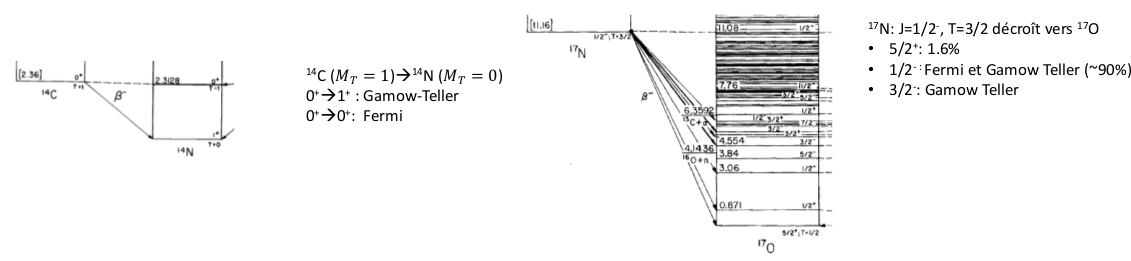
\includegraphics[scale=0.4]{ch6/image7}
	\captionof{figure}{A gauche ; deux transitions sont autorisée (soit purement l'une, soit purement l'autre). A
	droite ; plus compliqué à cause d'une grande densité de niveau.}
\end{center}



\subsection{Transition interdite}
Si les deux conditions ne sont pas satisfaites, il faut reconsidérer les précédentes approximations. Pour se faire,
partons de l'onde plane de l'électron
\begin{equation}
e^{i\vec k_e.\vec r} \approx \underbrace{1}_{1}+ \underbrace{i\vec{k_e}.\vec{r}}_{2}+
\underbrace{\frac{1}{2}(i\vec{k_e}.\vec{r})^2}_{3} + \dots
\end{equation}
\begin{enumerate}
\item Transition permise
\item Transition une fois interdite : $\pi_i\pi_f=-1, \Delta J = 0,\pm1, \pm2$
\item Transition deux fois interdite : $\pi_i\pi_f=+1, \Delta J = 0,\pm1, \pm2, \pm3$
\end{enumerate}\ 

Si les deux premiers sont interdits, il faut prendre le troisième et ainsi de suite. Chaque terme additionnel est
de plus en plus petit mais il faut en tenir compte car les dominants ne contribuent pas. Il existe un cas
extrêmement pathologique du $^{115}_{49}In(9/2^+)\to ^{115}_{50}Sn(1/2^+)$ où les quatre premiers termes sont
interdits. La probabilité de transition est donc très faible ce qui lui confère une longue durée de vie
($4.4\times 10^{14}$ ans).



\section{Probabilité de transition intégrée}
L'intégration de 
\begin{equation}
\frac{dW}{dE} = \dfrac{dW}{dT_e} = \frac{1}{2\pi^3}\frac{1}{\hbar(m_ec^2)^4}G_\beta^2cp_e(Q_\beta-T_e)^2(T_e+
m_ec^2)F(\pm Z,p_e)|M_{fi}|^2
\end{equation}
sur toutes les énergies électroniques donne la probabilité de transition intégrée. Celle-ci vaut
\begin{equation}
W = \frac{1}{2\pi^3}\frac{m_ec^2}{\hbar}G_\beta^2f(Q_{\beta},\pm Z)|M_{fi}|^2
\end{equation}
où $\DS f(Q_\beta, \pm Z) = \frac{c}{(m_ec^2)^5}\int_0^{Q_\beta} p_e(Q_\beta-T_e)^2(T_e+m_ec^2)F(\pm Z, p_e)dT_e$.\\


	\begin{wrapfigure}[9]{r}{6cm}
	\vspace{-8mm}
	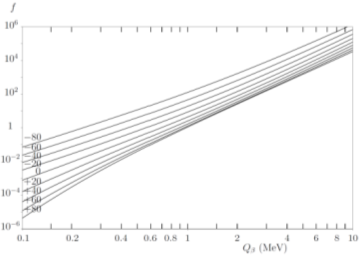
\includegraphics[scale=0.45]{ch6/image8}
	\captionof{figure}{ }
	\end{wrapfigure}
Il s'agit de l'\textit{intégrale de Fermi} (sans dimension). La dépendance en $Q_\beta$ est forte car le seuil 
est petit : peu d'énergie pour l'électron et le neutrino. On parle d'\textit{espace de phase}, soit l'ensemble des
états dans lequel on peut trouver le neutrino et l'électron. Forcément si $Q_\beta$ est petit, l'espace des phases
est petit et la probabilité de transition est petite (à gauche). Les durées de vie sont donc très variables et
il y a une différences entre $\beta^+$ et $\beta^-$.\\

Sachant que la demi-vie est donnée par $t_{1/2} = \ln 2/W$, on peut en déduire la valeur de $ft$
\begin{equation}
ft_{1/2} = \ln2\dfrac{2\pi^3\hbar}{m_ec^2G_\beta^2|M_{fi}|^2}
\end{equation}
Le temps de demi-vie à les dimension d'un temps, il est indépendant de $Q_\beta$ et ne dépend que de l'élément de
matrice nucléaire $M_{fi}$. Il se peut que $t_{1/2}$ varie de plusieurs ordre de grandeur. Si $\log_{10} ft_{1/2}$
vaut 3-6 la transition est permise, si 6-9 une fois interdite et si elle vaut 22.5 elle est quatre fois 
interdites.\\

Etudions le cas particulier d'une \textbf{transition entre deux états d'un même multiplet d'isospin}. Les parties
spatiales doivent être similaires ($M_{fi}$ maximum, transitions \textit{superpersmises}).  Considérons le 
cas très simple d'une transition $\beta^+$ où $J_i=0^+, T_i=1, M_{Ti}=-1, J_f=0^+, T_f=1,M_{Tf}=0$. Les 
transition de \textsc{Gamow-Teller} sont interdites ($J_i=J_f=0$), seulement \textsc{Fermi}. L'élément de matrice
nucléaire $|M_{fi}|^2\approx 2$ de sorte que $\log_10(ft)\approx 3$ (ordre de 3000s).

\newpage
\begin{center}
	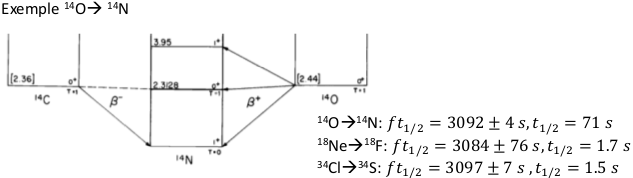
\includegraphics[scale=0.5]{ch6/image9}
	\captionof{figure}{Trois cas différent, trois état avec un même multiplet : les valeurs de $ft_{1/2}$ sont 
	comparables. Les durées de vies sont relativement différentes mais ça c'est à cause de la fonction $f$, 
	différentes dans chacun des cas.}
\end{center}








\section{Capture électronique}
La capture électronique est un phénomène qui rentre en compétition avec la radioactivité $\beta^+$ car elle 
produit un noyau dont la charge est diminuée d'une unité
\begin{equation}
^A_ZX_N + e^- \to ^A_{Z-1}Y^*_{N+1} + \nu
\end{equation}
où $Y^*$ est le noyau fille dans un état excité, causant une réorganisation du cortège électronique. Le seuil
de la capture électronique s'obtient - comme toujours - par bilan. Celui-ci vaut (on se souvient de la 
différence avec $\beta^+$ de $2m_ec^2$)
\begin{equation}
Q_{CE} = [M(Z,A)-M(Z-1,A)]c^2-B_e \approx Q_{\beta^+}+2m_ec^2
\end{equation}\ 

Il y a cependant des différences avec l'émission $\beta^+$ (charge $Z$ diminuée de 1) :
\begin{itemize}
\item[$\bullet$] Neutrinos monoénergétiques
\item[$\bullet$] Électron lié ((fait partie du cortège électronique)
\item[$\bullet$] Différence dans les densités d'états)
\end{itemize}\ 

En effet, les densités d'états changent et il faut en tenir compte
\begin{equation}
\rho = \frac{d\vec{k}}{dE} = k^2d\Omega\frac{dk}{dE}
\end{equation}
Dans un cas isotrope, on retrouve $\rho(E) = \frac{4\pi E_\nu^2}{(\hbar c)^3}$. Notons aussi la 
fonction d'onde électronique
\begin{equation}
\Psi_e(0) = \pi^{-1/2}\left(\dfrac{Z}{a_0}\right)^{3/2}
\end{equation}
où $n=1$ (orbite) et $a_0 = \hbar^2/(m_ee^2)$ est le rayon de \textsc{Bohr}.\\


	\begin{wrapfigure}[8]{r}{4cm}
	\vspace{-8mm}
	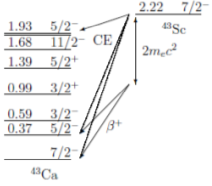
\includegraphics[scale=0.5]{ch6/image10}
	\captionof{figure}{Niveau au dessus de $2m_ec^2$, seulement CE. Cas en dessous : compétition.}
	\end{wrapfigure}

On peut en déduire la probabilité de capture électronique
\begin{equation}
W_{CE} = \frac{1}{\pi^2}(\alpha Z)^3\dfrac{E_\nu^2}{\hbar m_ec^2}G_\beta^2|M_{fi}|^2
\end{equation}
On observe que $Q_{CE}$ est de l'ordre de $E_\nu$, la dépendance en $Q_{CE}$ est donc faible au 
contraire de la radioactivité $\beta$\footnote{Pas compris, quelqu'un peut expliciter?}.\\

Étant donné qu'il y a deux phénomènes possibles, il faut les comparer. On définit alors le
\textit{rapport de branchement} défini comme le rapport entre la probabilité d'avoir $\beta^+$ sur 
la probabilité d'avoir une capture électronique. Ce rapport est assez facile à calculer : les 
$|M_{fi}|$ se simplifie, on connaît les masses, seuils, \dots Deux cas sont possibles :
\begin{enumerate}
\item Si $Q_{CE} < 2m_ec^2$
\begin{equation}
\frac{W_{\beta^+}}{W_{CE}} =0
\end{equation}
Puisque $Q_{CE} = Q_{\beta^+}+2m_ec^2$, seule la capture électronique est possible
\item Si $Q_{CE} > 2m_ec^2$
\begin{equation}
\frac{W_{\beta^+}}{W_{CE}} =\dfrac{f(Q_{\beta^+},Z)}{2\pi(\alpha Z)^3}\left(\dfrac{m_ec^2}{Q_{CE}}\right)^2
\end{equation}
Il y a compétition entre la capture électronique et $\beta^+$ sauf si $f(Q_{\beta^+},Z)$ est petit
(et donc $Q_{\beta^+}$ petit). Souvent ce rapport est grand, $\beta^+$ est donc favorisé. Mais il ne faut 
donc pas oublier le cas où l'intégrale de \textsc{Fermi} est petite causant un seuil petit : un petit seuil favorise la compétition.
\end{enumerate}\ 


\section{Autres processus}
Il en existe principalement deux 
\begin{enumerate}
\item Capture de neutrinos
\item Radioactivité $\beta$ double
\end{enumerate}\ 

Intéressons-nous aux deuxième cas à travers deux exemples. \\

\textsc{Transition $\beta$ interdite}\ \\

	\begin{wrapfigure}[12]{r}{10cm}
	\vspace{-8mm}
	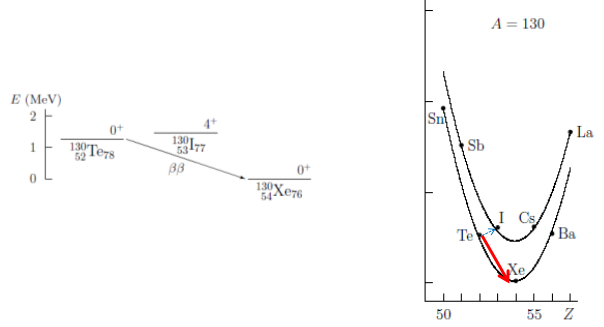
\includegraphics[scale=0.5]{ch6/image11}
	\captionof{figure}{ }
	\end{wrapfigure}
	
La transition $\beta$ pour le $^130$Te est interdite (probabilité de 0\%) mais pas la transition 
$2\beta$ (probabilité de 100\%). Ceci s'explique par le fait que la transition (pour $A=130$) du Te 
vers I est interdite (masse plus grande). La seule façon de "redescendre la parabole" est d'aller vers 
le Xe, ce qui n'est possible que par émission $\beta\beta$ (désintégration $\beta$ double). Le temps de
demi-vie est cependant de $5\times 10^23$ ans.\\







\textsc{Transition $\beta$ défavorisée}
Soit le $^{48}$Ca. La transition $\beta$ n'est pas totalement absente mais c'est la $\beta$ double qui fait
tout le travail. La durée de vie bien plus grande que l'âge de l'Univers. On l'utilise pour obtenir des éléments
superlourd (projectile pour crée ces éléments). Voir \textit{slide 99}, pas la place pour mettre l'image 
ici \textit{pfpfpfpf}.